\chapter{Présentation du cadre de projet}

\section*{Introduction}
Dans ce chapitre, nous présenterons une description générale de l’organisme d’accueil, CIH BANK, d’un point de vue organisationnel. Nous aborderons ensuite l'étude de l'existant, le choix du modèle de développement ainsi que le planning prévisionnel du projet, afin de mieux contextualiser notre travail de fin d'études.

% =========================
\section{Présentation de l'organisme d'accueil}

Le Crédit Immobilier et Hôtelier (CIH), plus communément appelé CIH BANK, est une banque marocaine dont le siège social se trouve à Casablanca. Historiquement connu pour son activité dans le secteur de l’immobilier, le CIH propose désormais des services bancaires variés à ses clients, particuliers et professionnels.

CIH BANK a été fondée en 1920 sous le nom de Caisse de Prêts Immobiliers du Maroc (CPIM). En 1967, le groupe a étendu son activité au secteur hôtelier et a changé de nom pour devenir le Crédit Immobilier et Hôtelier.

\begin{table}[h]
\centering
\begin{tabular}{|l|l|}
\hline
Création & 1920 \\
\hline
Fondateur & L’État marocain \\
\hline
Introduction en bourse & 1967 \\
\hline
Forme juridique & Société anonyme \\
\hline
Slogan & La banque de demain dès aujourd’hui \\
\hline
Siège social & 187, Avenue Hassan II, Casablanca, Maroc \\
\hline
Président Directeur Général (PDG) & Lotfi SEKKAT \\
\hline
Société mère & Caisse de Dépôt et de Gestion \\
\hline
Effectif & 2 181 \\
\hline
Site web & www.cihbank.ma \\
\hline
\end{tabular}
\caption{Informations générales sur le groupe CIH BANK}
\end{table}

% =========================
\subsection{Missions de CIH BANK}

Spécialisé dans le financement immobilier et hôtelier, le CIH est un partenaire historique des pouvoirs publics en matière de financement du logement depuis 1920. La banque finance les promoteurs immobiliers au Maroc par deux canaux complémentaires. En amont, elle assure le financement des promoteurs publics et privés pour l'acquisition, la viabilisation des terrains et la construction des programmes immobiliers. En aval, elle octroie des crédits au logement pour les particuliers acquéreurs, tout en proposant divers services et produits bancaires adaptés à sa clientèle.

% =========================
\subsection{Secteurs d’activité}

Le groupe CIH BANK et ses filiales offrent une vaste gamme de produits et de services couvrant les besoins de ses clients particuliers et professionnels. Ces services incluent les opérations bancaires classiques, les prêts aux particuliers (tels que les prêts immobiliers et crédits à la consommation), ainsi que le financement d'entreprises (via des prêts d'investissement, d'exploitation et du crédit-bail). Le groupe intervient également dans le domaine de l'assurance et dispose d'une salle des marchés active.

% =========================
\subsection{Filiales}

Afin de diversifier ses activités, le groupe CIH BANK s'appuie sur plusieurs filiales spécialisées. On y retrouve SOFAC pour les solutions de crédit, SOFASSUR et CIH Courtage pour les services d'assurance, ainsi que Maroc Leasing, qui propose des solutions de financement pour les véhicules, le BTP, l'immobilier et la santé. Le groupe est également présent dans la finance participative avec Umnia Bank, et dans la gestion d'Organismes de Placement Collectif Immobilier (OPCI) via AJAR INVEST, dont CIH BANK détient 40 \% des parts.

% =========================
\subsection{Actionnariat}

La répartition du capital du groupe CIH BANK est présentée dans le tableau \ref{tab:actionnariat} :

\begin{table}[h]
\centering
\caption{Répartition du capital de CIH BANK}
\label{tab:actionnariat}
\begin{tabular}{|l|c|}
\hline
\textbf{Actionnaire} & \textbf{Part} \\
\hline
Massira Capital Management & 55,66 \% \\
\hline
Flottant en bourse & 16,37 \% \\
\hline
Atlanta Sanad & 11,61 \% \\
\hline
Caisse de Dépôt et de Gestion (CDG) & 6,69 \% \\
\hline
Régime Collectif d’Allocation de Retraite (RCAR) & 5,21 \% \\
\hline
Personnel de la banque & 4,36 \% \\
\hline
Groupe Holmarcom & 0,12 \% \\
\hline
\end{tabular}
\end{table}

% =========================
\subsection{Chiffres clés}

La figure \ref{fig:chiffres} présente les chiffres clés de CIH BANK.

\begin{figure}[h]
    \centering
    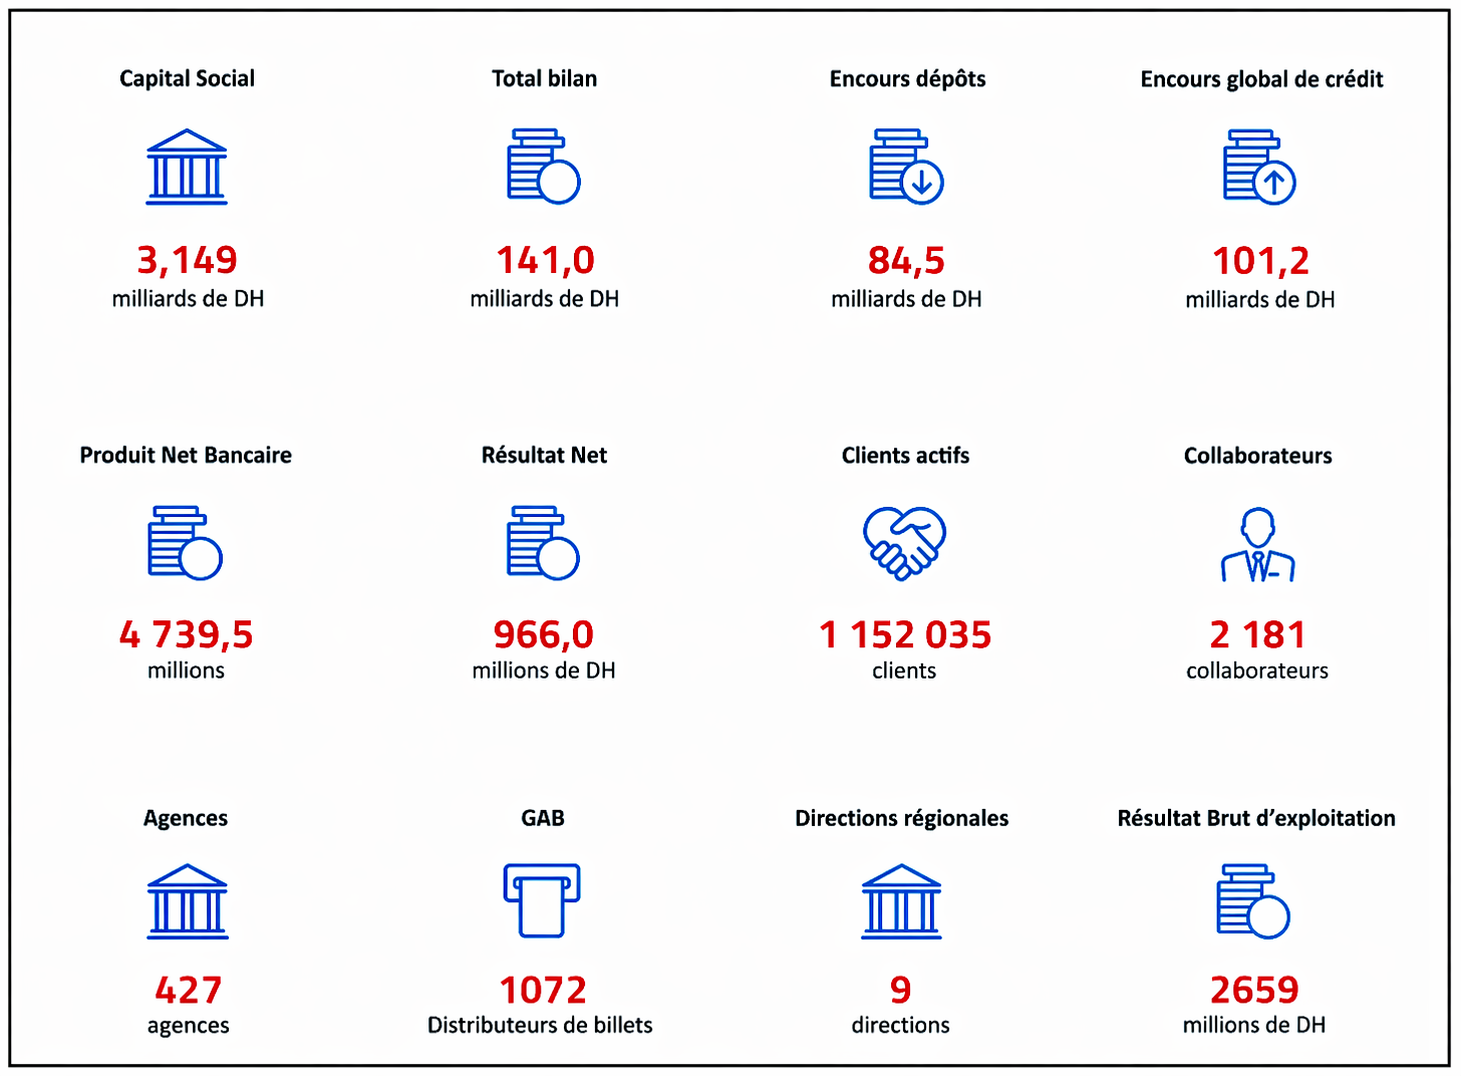
\includegraphics[width=0.8\textwidth]{figures/chiffresCles.png}
    \caption{Chiffres clés de CIH BANK (31/12/2024)}
    \label{fig:chiffres}
\end{figure}

Les chiffres clés de CIH BANK reflètent la situation financière et opérationnelle de l’institution. Avec un capital social de 3,149 milliards de dirhams et un total bilan de 141 milliards de dirhams, la banque dispose d’une base financière significative. L’encours des dépôts s’élève à 84,5 milliards de dirhams, tandis que l’encours global de crédit atteint 101,2 milliards de dirhams. Le produit net bancaire est de 4 739,5 millions de dirhams, avec un résultat net de 966 millions de dirhams et un résultat brut d’exploitation de 2 659 millions de dirhams. La banque compte plus de 1,15 million de clients actifs, 2 181 collaborateurs, 427 agences, 1 072 guichets automatiques et 9 directions régionales. Ces indicateurs fournissent une vue d’ensemble de l’activité, de la structure et des résultats financiers de l’institution.

% =========================
\subsection{Organigramme}

\subsubsection{Structure hiérarchique de CIH BANK}

La structure hiérarchique de CIH BANK s'articule autour d'une direction générale pilotée par le Président Directeur Général, appuyée par des fonctions de support stratégique et de contrôle (Audit, Conformité, Risques, Capital Humain, etc.) ainsi que diverses fonctions rattachées. L'activité commerciale et opérationnelle de la banque est quant à elle répartie en plusieurs pôles métiers majeurs : la Banque des Particuliers et Professionnels, la Banque de l’Entreprise et de l’Immobilier, la Banque de l’Investissement, le Financement \& Recouvrement, et les Services à la Clientèle \& Réseaux.

Parmi ces différentes directions, notre attention se porte plus particulièrement sur l'entité technologique qui encadre notre organisme d'accueil :

\paragraph*{Fonctions technologiques et data}

Au niveau des fonctions technologiques et de gestion de la donnée, le pôle Services Technologiques et Opérations englobe la Sécurité des Systèmes d’Information, la Qualité, ainsi que le Pôle Systèmes d’Information. C'est au sein de la direction Data Management \& Intelligence Artificielle de ce même pôle que se trouve le Data Office, l'entité d'accueil de notre projet de fin d'études.

L'organigramme global de CIH BANK est illustré dans la figure \ref{fig:organigramme} ci-dessous.

\begin{figure}[H]
    \centering
    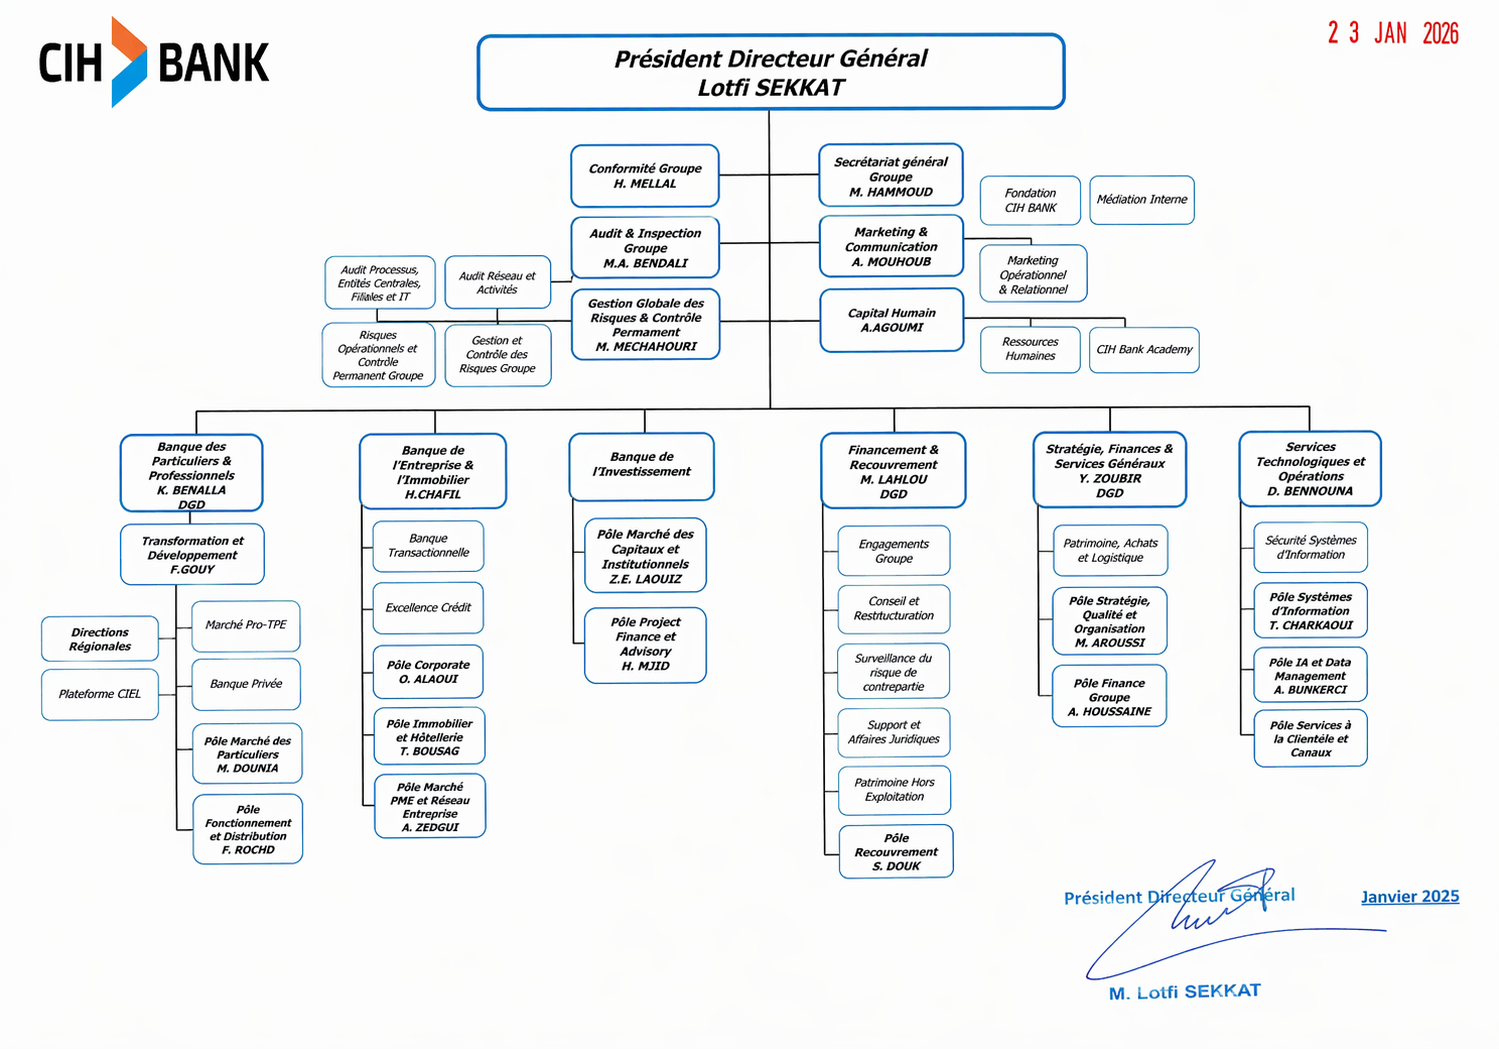
\includegraphics[angle=90, width=\textwidth, height=0.8\textheight, keepaspectratio]{figures/Organigramme.png}
    \caption{Organigramme de CIH BANK}
    \label{fig:organigramme}
\end{figure}

% =========================
\subsection{Data Office}

Dans le cadre de notre stage, nous avons intégré le Data Office de CIH BANK, une entité dédiée à la gestion, au traitement et à la valorisation des données de la banque.

Le Data Office est aujourd’hui rattaché au pôle Services Technologiques et Opérations, plus précisément au sein de la direction Data Management et Intelligence Artificielle. Cette organisation reflète l’importance stratégique accordée à la donnée dans le pilotage des activités de la banque.

Cette entité regroupe plusieurs profils complémentaires intervenant sur l’ensemble du cycle de vie de la donnée. Les \textit{Data Engineers} sont en charge de l’ingestion, du traitement et de la mise à disposition des données. Ils collaborent étroitement avec les \textit{Data Analysts}, responsables de l’analyse et de la production d’indicateurs décisionnels, ainsi qu'avec les \textit{Data Scientists}, spécialisés dans la modélisation avancée et l’analyse prédictive. Enfin, l’équipe \textit{Data Management} assure la gouvernance transversale, la qualité et la structuration des données au sein de la banque.

Les données sont collectées à partir des différents systèmes opérationnels de la banque, puis intégrées et centralisées au sein d’un Data Lake. Elles sont ensuite transformées et mises à disposition pour répondre aux besoins analytiques, réglementaires et métiers.

Dans ce cadre, le Data Office joue un rôle central dans la mise en place des pratiques de gestion de la qualité des données.


% =========================
\section{Étude de l'existant}

\subsection{Description de l'existant}

\subsubsection*{Contexte et enjeux de la qualité des données bancaires}
Dans l'écosystème financier contemporain, la transition vers une économie numérique a redéfini la nature des institutions bancaires. La donnée n'est plus un simple sous-produit de l'activité transactionnelle, mais s'impose comme une infrastructure essentielle sur laquelle reposent l'évaluation des risques, les décisions stratégiques, et une conformité réglementaire extrêmement stricte. Au Maroc, cette conformité s'articule prioritairement autour de la protection des données à caractère personnel, régie par la loi 09-08 de la CNDP (Commission Nationale de contrôle de la protection des Données à caractère Personnel). S'y ajoute le respect du RGPD européen pour la clientèle résidant en Europe, ainsi que d'autres normes internationales liées aux risques (ex: BCBS 239).
Sur le plan économique, le coût de la non-qualité est très élevé. La « règle de dix » (\textit{Rule of Ten}) stipule qu'il coûte dix fois plus cher de corriger une donnée en aval que de la valider directement à la source. Une gouvernance proactive apporte une valeur mesurable : optimisation des fonds propres, efficacité opérationnelle et sécurisation des décisions basées sur l'intelligence artificielle.

\subsubsection*{Le domaine Tiers : Cartographie et données}
Historiquement, la vérification de la qualité des données au sein de CIH BANK était un processus réactif déclenché sur demande, ce qui a motivé la création de l'entité Data Management (DM). Notre projet s'inscrit dans cette volonté d'amélioration continue et cible plus particulièrement le \textbf{Référentiel Tiers}. Ce référentiel regroupe l'ensemble des informations relatives aux personnes physiques et morales en relation avec la banque.

Dans le cadre de l'ingestion des données vers le Data Lake, l'équipe travaille sur plus d'une dizaine de tables du domaine Tiers. À titre d'illustration, les tables principales extraites du système opérant Oracle NOVA (\texttt{CCM}) qui structurent notre périmètre de base sont : \texttt{identity} (pièces d'identité), \texttt{legalentity} (personnes morales), \texttt{person} (statut client), \texttt{professionaldescription} (caractéristiques professionnelles), \texttt{jobs} (catégories socio-professionnelles CSP), ainsi que la table centrale \textbf{\texttt{np\_description}} (Natural Person Description) regroupant les données d'état civil et les informations KYC pour les personnes physiques.

Bien que le pipeline automatisé de qualité de données déployé couvre l'ensemble du domaine Tiers (soit une quinzaine de tables issues de NOVA), \textbf{pour des soucis de clarté et d'illustration, les implémentations techniques et les règles de Data Quality présentées dans la suite de ce rapport se focaliseront particulièrement sur les tables \texttt{np\_description} et \texttt{jobs}}. Ces tables sont éminemment stratégiques : \texttt{np\_description} concentre les données KYC indispensables à l'identification réglementaire du client (nom, prénom, date de naissance, genre, nationalité, etc.), tandis que \texttt{jobs} contient des informations essentielles pour la catégorisation socio-professionnelle (CSP).

\subsubsection*{Architecture et pipeline de données}
L'ensemble des données ingérées au sein de CIH BANK, incluant celles du domaine Tiers, transite par une plateforme robuste centralisée s'appuyant sur une infrastructure Big Data de pointe. Tout l'écosystème analytique repose sur ce système unifié pour le traitement et la valorisation de la donnée.

\begin{figure}[H]
\centering
\includegraphics[width=0.95\textwidth]{figures/Architecture et pipeline de données.png}
\caption{Architecture matérielle Big Data}
\label{fig:architecture_big_data}
\end{figure}

L'architecture matérielle et logicielle de cette plateforme de production s'articule autour d'un \textbf{cluster Cloudera et Dremio} composé de 8 nœuds (3 Masters, 3 Workers, 2 Gateways). Le flux global des données, de la source à l'exploitation, suit un cycle de vie standardisé en plusieurs étapes :

\paragraph{1. Ingestion :} Les données brutes issues des systèmes opérants (Oracle NOVA, PowerCard, etc.) sont ingérées massivement via des scripts \textbf{Apache Sqoop} organisés par domaine métier. Les tables sont stockées au format \textbf{ORC} dans la zone RAW de Hive via HCatalog. L'authentification aux sources s'effectue par \textbf{Kerberos} (\texttt{kinit} avec keytab).

\paragraph{2. Transformation :} Des pipelines PySpark packagés sous forme de fichiers \textbf{Wheel} (\texttt{.whl}), construits via le gestionnaire \textbf{PDM}, effectuent le nettoyage, le renommage des colonnes et l'enrichissement des données brutes pour les charger dans la zone de STAGING. Chaque écriture est tracée par une colonne d'audit \texttt{batch\_time}.

\paragraph{3. Virtualisation et Métadonnées :} Le moteur de données Dremio se connecte aux catalogues (Hive Metastore) pour virtualiser les tables. Il offre une couche sémantique puissante permettant de croiser et d'interroger les données sans les dupliquer.

\paragraph{4. Exposition et Datamarts :} Les données transformées sont consolidées et exposées sous forme de Datamarts (ou vues métiers spécifiques). Ces ensembles de données prêts à l'emploi alimentent les outils de restitution (Tableau) pour répondre aux besoins analytiques des métiers.

\subsection{Critique de l'existant}
Bien que cette infrastructure de production Cloudera soit robuste, l'absence d'un contrôle automatisé de la qualité des données en amont pose plusieurs problèmes majeurs transverses à l'ensemble des tables du domaine Tiers. Pour illustrer l'impact de ces problèmes, nous prenons l'exemple des tables \texttt{np\_description} et \texttt{jobs}, qui contiennent des données KYC et CSP particulièrement sensibles concernant les personnes physiques :

\paragraph{Absence de validation à la source :} Les données transitent vers Dremio sans aucune validation intermédiaire. Des incohérences flagrantes persistent, comme des discordances entre le genre et la civilité du client, ou des dates de naissance remplies par défaut.

\paragraph{Risques de non-conformité réglementaire :} L'absence ou l'invalidité de certains champs critiques, tels que l'identifiant FATCA pour les clients concernés, expose la banque à des risques réglementaires et à d'éventuelles sanctions.

\paragraph{Démarche réactive et manuelle :} Lorsqu'une anomalie est repérée par les métiers en bout de chaîne, la réconciliation implique asynchronement plusieurs équipes pour des corrections curatives chronophages, créant ainsi des processus inefficaces.

\paragraph{Manque de traçabilité et d'historisation :} Aucune métrique n'est historisée dans le temps. Les Data Stewards ne disposent d'aucun outil pour prioriser ou surveiller la santé des données KYC au quotidien.

\subsection{Solution proposée}
Pour pallier ces limites, nous proposons de concevoir et d'implémenter un \textbf{pipeline automatisé de contrôle de la qualité des données} couvrant l'ensemble du périmètre Tiers, intégré directement dans la zone RAW de l'infrastructure Hadoop. La solution technique s'articule autour de trois piliers majeurs :

\paragraph{Automatisation native via Soda Core :} L'intégration de la bibliothèque Soda Core au sein des workflows Airflow existants permet de valider systématiquement les données KYC (exhaustivité, unicité, validité de format, cohérence croisée) dès leur ingestion.

\paragraph{Approche proactive et détection précoce :} En signalant les anomalies dès la zone RAW, nous empêchons l'exploitation de données erronées par les couches analytiques aval, appliquant ainsi le principe de la \textit{Rule of Ten}.

\paragraph{Monitoring centralisé et restitution décisionnelle :} Les résultats des contrôles et les anomalies consolidées sont persistés dans des tables Hive dédiées. Un tableau de bord interactif est ensuite construit pour offrir aux Data Stewards une vue claire de la santé des tables du référentiel, tout en garantissant la stricte anonymisation des données personnelles.

\paragraph{Fondation pour l'Intelligence Artificielle (\textit{Data Readiness for AI}) :} Dans le secteur bancaire, la fiabilité des modèles prédictifs et des algorithmes d'apprentissage automatique (tels que le scoring de risque de crédit, la détection des fraudes ou la segmentation client) est strictement conditionnée par la qualité des données en entrée (\textit{Garbage In, Garbage Out}). En garantissant la complétude et la cohérence des variables fondamentales KYC et CSP dès leur arrivée dans le Data Lake, notre pipeline assure la robustesse des données destinées à alimenter les pipelines de Machine Learning de la banque.

Cette solution permet d'améliorer la gouvernance globale des données du domaine Tiers tout en optimisant le temps de traitement des anomalies.

\section{Choix du modèle de développement}

Pour mener à bien ce projet, nous avons adopté une démarche \textbf{Agile inspirée du framework Scrum, adaptée aux spécificités de l'ingénierie Big Data}. La complexité de l'écosystème distribué et l'étendue du domaine Tiers ont motivé un découpage itératif par livrables fonctionnels (\textit{Minimum Viable Products} et \textit{Proof of Concepts}), permettant d'éprouver et de valider les règles de qualité de manière progressive, table par table.

Sur le plan opérationnel, cette démarche s'est articulée autour d'un rythme adapté : des synchronisations hebdomadaires (\textit{Weekly standups}) avec le \textit{Delivery Manager} pour piloter l'avancement des \textit{backlogs} individuels et lever les verrous techniques, associées à des points de validation réguliers avec le \textit{Data Steward} (agissant en tant que \textit{Product Owner} métier). Cette organisation a assuré une forte réactivité face aux contraintes de l'infrastructure Cloudera tout en maintenant un alignement continu avec les priorités métiers de la banque.

% =========================
\section{Planning prévisionnel}

Afin de mener à bien ce projet au sein du Data Office de CIH BANK, nous avons défini un planning de travail couvrant une période de six mois, du \textbf{9 février au 9 août 2026}. 

Contrairement à un projet classique, l'avancement n'a pas été strictement linéaire. Les deux premiers mois ont été presque exclusivement dédiés à la compréhension fonctionnelle, technique, et à la documentation détaillée de l'architecture existante. Par la suite, les phases de conception, de réalisation des POCs, et de tests se sont superposées de manière itérative, accompagnées de réunions continues avec les métiers.

La figure \ref{fig:gantt} ci-dessous illustre ce déroulement sous forme d'un diagramme de Gantt, mettant en évidence la phase initiale de documentation, le cycle itératif de développement, et l'implication constante des acteurs métiers.

\begin{figure}[H]
    \centering
    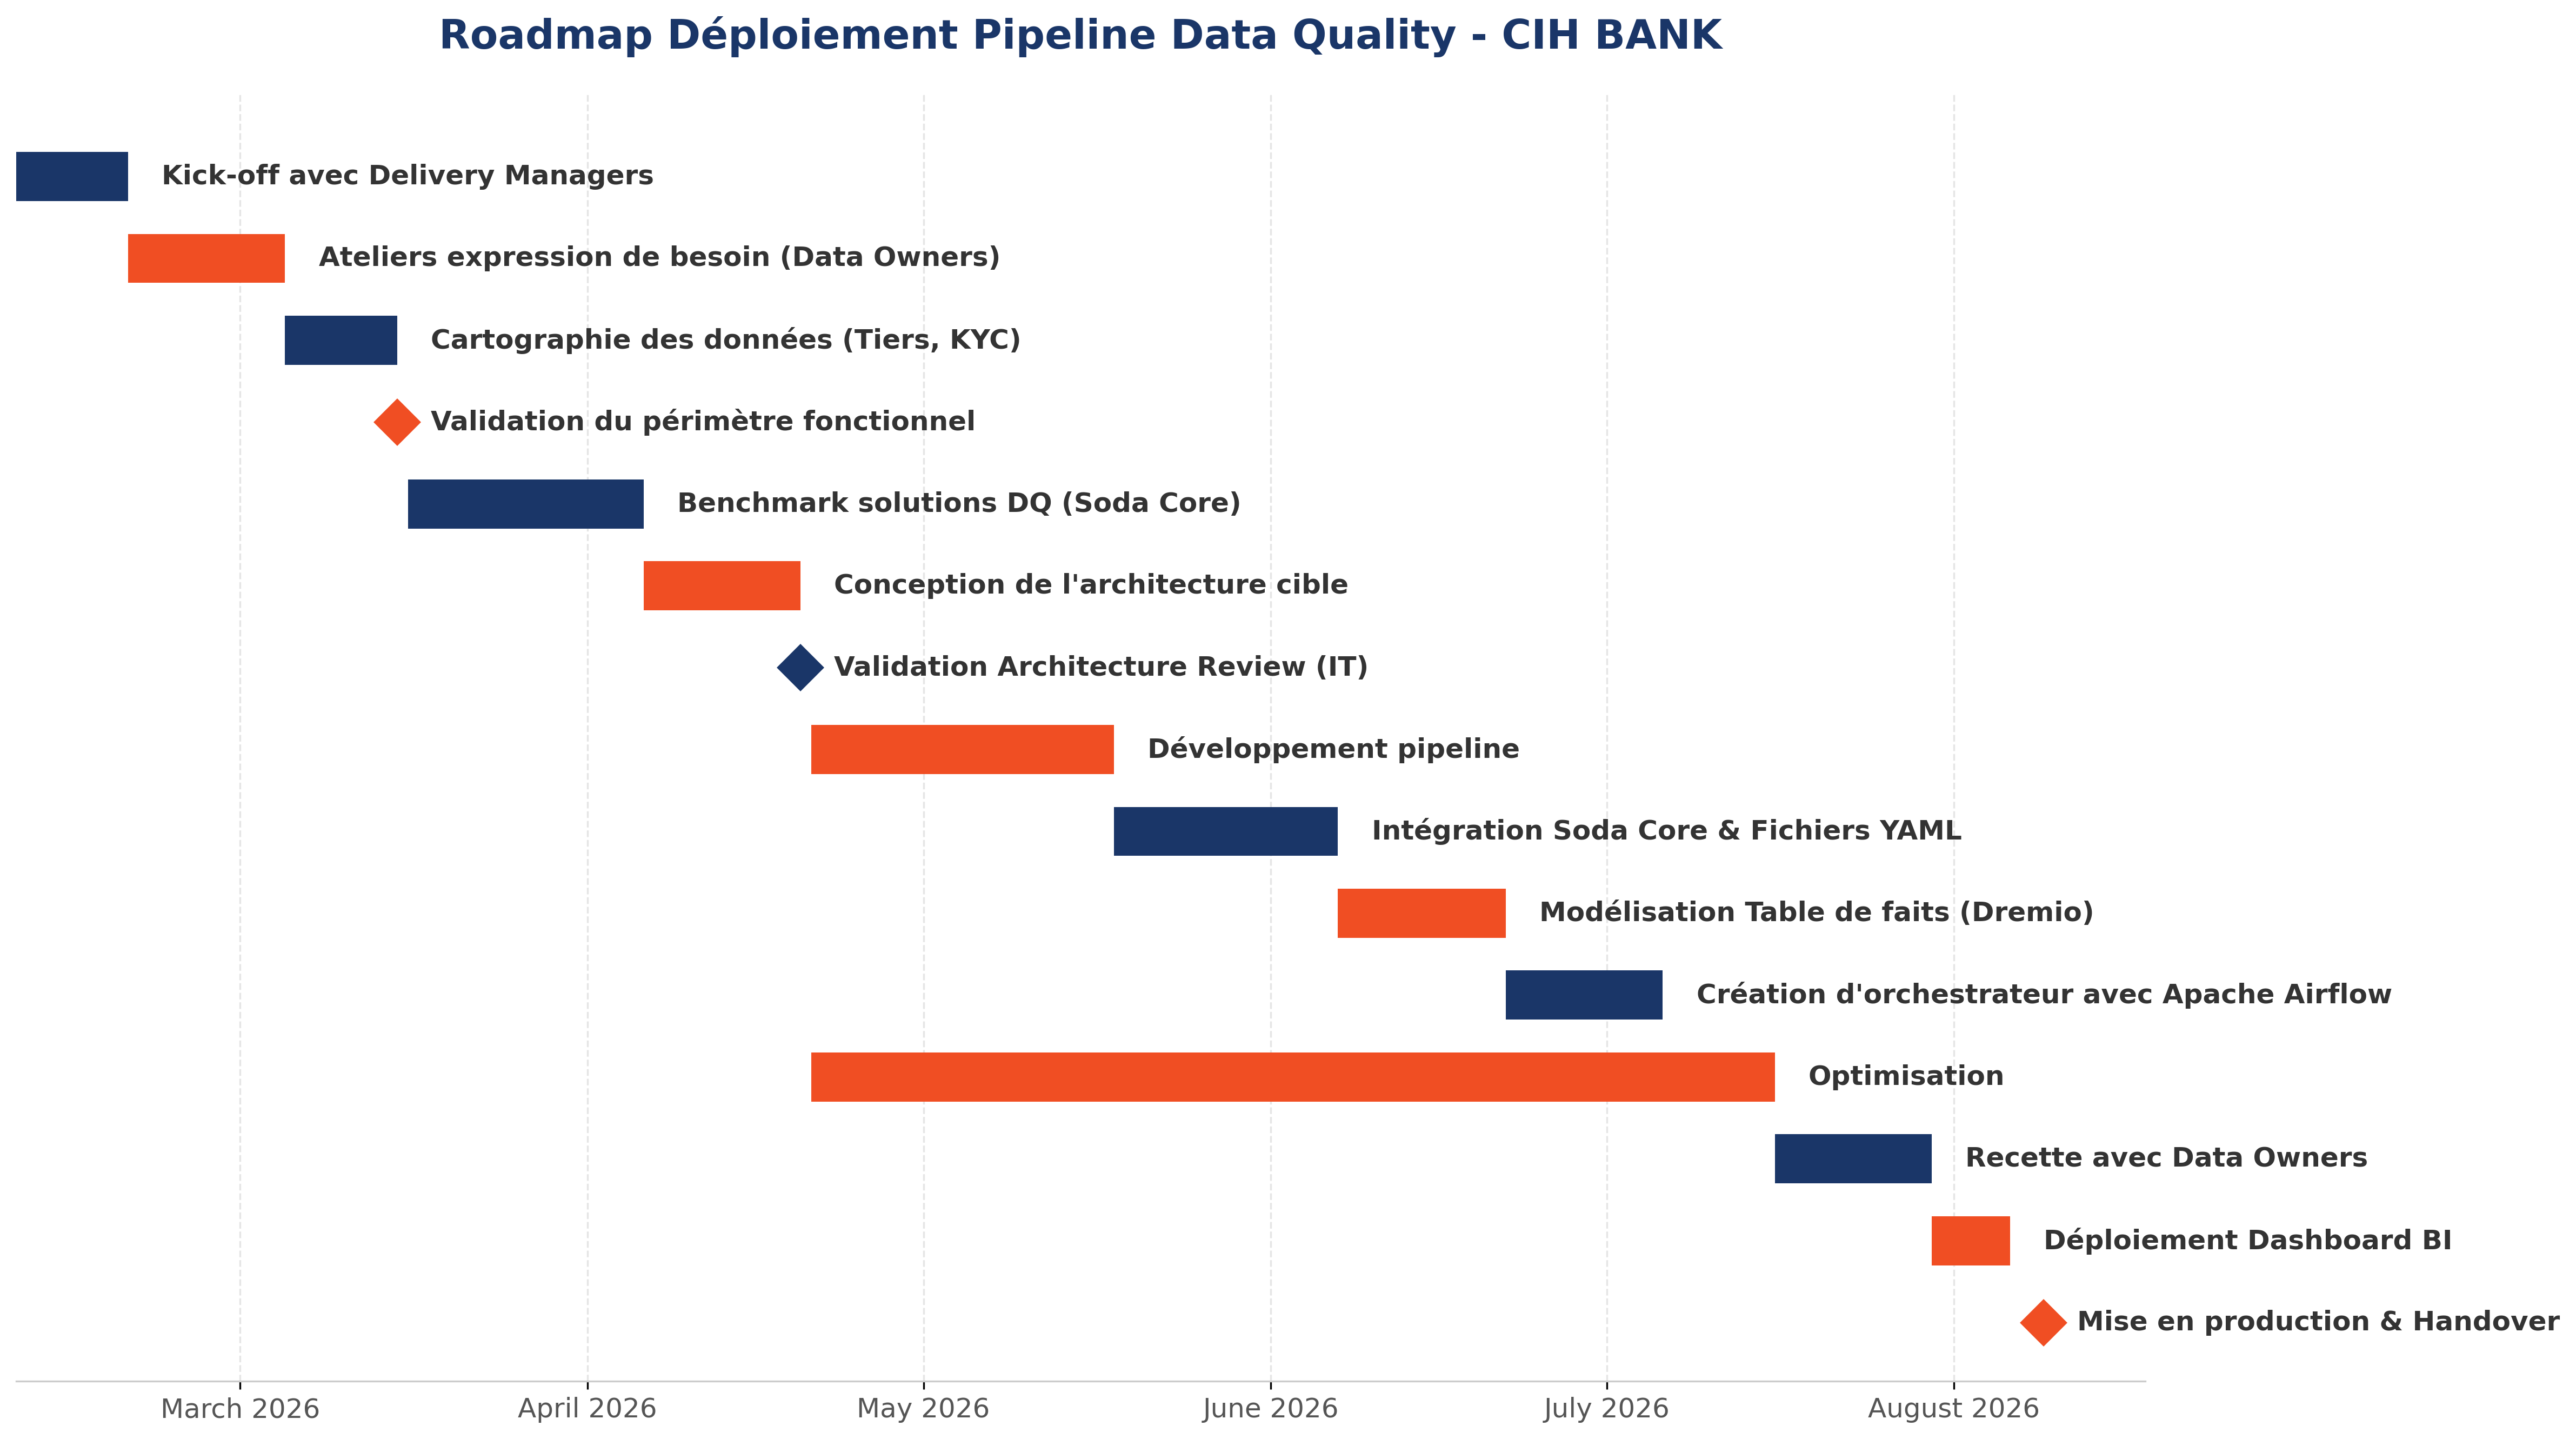
\includegraphics[width=1.0\textwidth]{figures/Gantt_CIH_Bank_Final.png}
    \caption{Planning prévisionnel du projet}
    \label{fig:gantt}
\end{figure}

% =========================
\section*{Conclusion}

Pour conclure, CIH BANK est une institution bancaire marocaine majeure, fortement structurée et engagée dans la valorisation de la donnée à travers son Data Office. L'étude de l'existant a permis de mettre en évidence les processus actuels de gestion des données et leurs limites, ce qui justifie la nécessité d'un pipeline automatisé de contrôle qualité. Ces éléments constituent la base de notre projet et nous permettent d'entamer sereinement la phase de spécification des besoins dans le chapitre suivant.
